\documentclass[12pt, a4paper]{article}

\usepackage[utf8]{inputenc}
\usepackage[T1]{fontenc}
\usepackage{geometry}
\geometry{margin=1in}
\usepackage{graphicx}
\usepackage{booktabs}
\usepackage{array}
\usepackage{hyperref}
\usepackage{amsmath}
\usepackage{enumitem}
\usepackage{float}
\usepackage{caption}
\usepackage{tabularx}
\usepackage{tikz}
\usetikzlibrary{shapes.geometric, arrows.meta, positioning, fit, backgrounds}
\usepackage{xcolor}

\definecolor{reddit}{HTML}{FF4500}
\definecolor{gdelt}{HTML}{4285F4}
\definecolor{tiktok}{HTML}{00F2EA}

\title{
  \textbf{Multiplatform Narrative Analysis of Venezuela--US Relations:}\\[6pt]
  \Large Integrating Social Media, News, and AI-Driven Intelligence\\[12pt]
  \large Methodology Report
}
\author{
  Hunjun Shin, Rich Goodier, Ameir El Ouadi\\
  \textit{Northeastern University}
}
\date{March 2026}

\begin{document}
\maketitle

%===================================================================
\section{Introduction}
%===================================================================

This report presents the methodology behind a multiplatform narrative analysis system designed to track, analyze, and visualize online discourse surrounding Venezuela--US bilateral relations from 2013 to 2026. The system ingests data from three heterogeneous sources---Reddit, GDELT news articles, and TikTok---and applies a pipeline of natural language processing (NLP) techniques including transformer-based sentiment analysis, dynamic topic modeling, and density-based semantic clustering. An LLM-powered intelligence layer synthesizes cross-platform findings into analyst-grade reports and supports interactive question-answering.

The following sections detail each stage of the pipeline: problem formulation (\S\ref{sec:problem}), data collection (\S\ref{sec:data}), model selection (\S\ref{sec:models}), training and development (\S\ref{sec:training}), and evaluation (\S\ref{sec:evaluation}).

% --- Architecture Diagram ---
\begin{figure}[H]
\centering
\resizebox{\textwidth}{!}{%
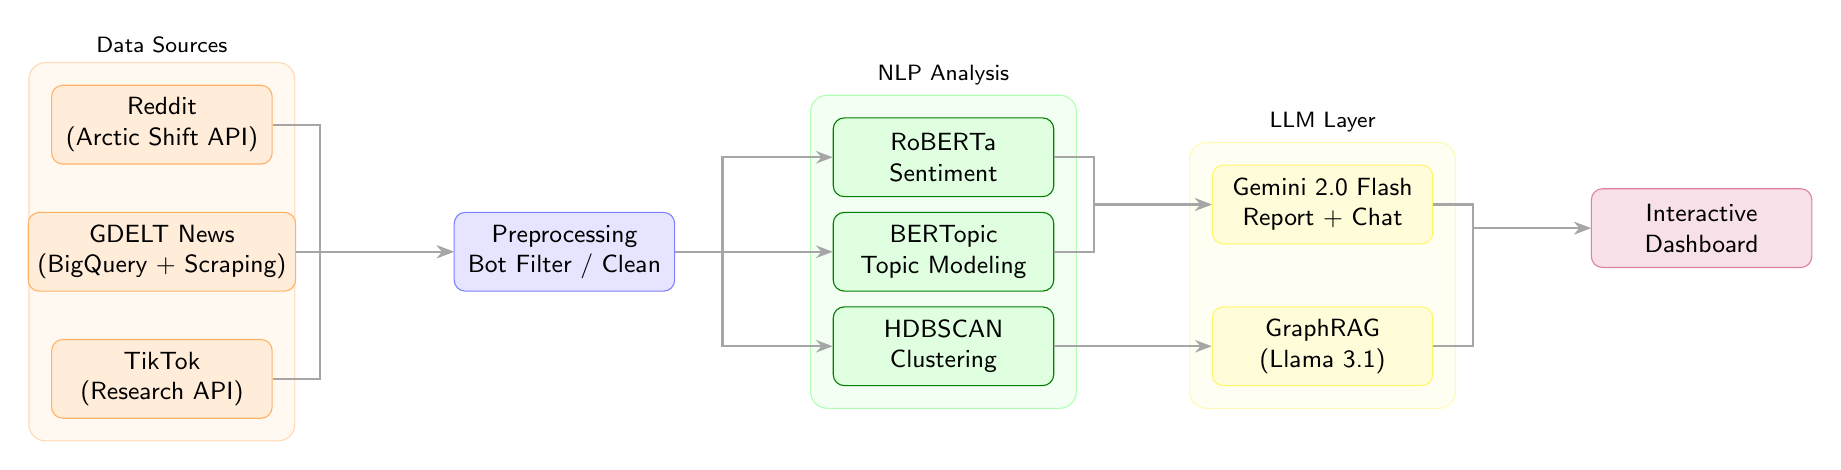
\begin{tikzpicture}[
    node distance=1.2cm and 1.6cm,
    box/.style={rectangle, draw, rounded corners=4pt, minimum height=1cm,
                minimum width=2.8cm, align=center, font=\small\sffamily},
    data/.style={box, fill=orange!15, draw=orange!60},
    proc/.style={box, fill=blue!10, draw=blue!50},
    model/.style={box, fill=green!12, draw=green!50!black},
    output/.style={box, fill=purple!12, draw=purple!50},
    arr/.style={-{Stealth[length=6pt]}, thick, gray!70},
  ]
  \node[data] (reddit)  {Reddit\\(Arctic Shift API)};
  \node[data, below=0.6cm of reddit] (gdelt) {GDELT News\\(BigQuery + Scraping)};
  \node[data, below=0.6cm of gdelt] (tiktok) {TikTok\\(Research API)};
  \node[proc, right=2cm of gdelt] (preproc) {Preprocessing\\Bot Filter / Clean};
  \node[model, right=2cm of preproc, yshift=1.2cm] (sentiment) {RoBERTa\\Sentiment};
  \node[model, right=2cm of preproc] (bertopic) {BERTopic\\Topic Modeling};
  \node[model, right=2cm of preproc, yshift=-1.2cm] (cluster) {HDBSCAN\\Clustering};
  \node[model, right=2cm of bertopic, yshift=0.6cm, fill=yellow!15, draw=yellow!60] (gemini) {Gemini 2.0 Flash\\Report + Chat};
  \node[model, right=2cm of bertopic, yshift=-1.2cm, fill=yellow!15, draw=yellow!60] (graphrag) {GraphRAG\\(Llama 3.1)};
  \node[output, right=2cm of gemini, yshift=-0.3cm] (dashboard) {Interactive\\Dashboard};
  \draw[arr] (reddit.east) -- ++(0.6,0) |- (preproc.west);
  \draw[arr] (gdelt.east) -- (preproc.west);
  \draw[arr] (tiktok.east) -- ++(0.6,0) |- (preproc.west);
  \draw[arr] (preproc.east) -- ++(0.6,0) |- (sentiment.west);
  \draw[arr] (preproc.east) -- (bertopic.west);
  \draw[arr] (preproc.east) -- ++(0.6,0) |- (cluster.west);
  \draw[arr] (sentiment.east) -- ++(0.5,0) |- (gemini.west);
  \draw[arr] (bertopic.east) -- ++(0.5,0) |- (gemini.west);
  \draw[arr] (cluster.east) -- ++(0.5,0) |- (graphrag.west);
  \draw[arr] (gemini.east) -- ++(0.5,0) |- (dashboard.west);
  \draw[arr] (graphrag.east) -- ++(0.5,0) |- (dashboard.west);
  \begin{pgfonlayer}{background}
    \node[fit=(reddit)(tiktok), inner sep=8pt, fill=orange!5, draw=orange!30,
          rounded corners=6pt, label={[font=\footnotesize\sffamily]above:Data Sources}] {};
    \node[fit=(sentiment)(cluster), inner sep=8pt, fill=green!5, draw=green!30,
          rounded corners=6pt, label={[font=\footnotesize\sffamily]above:NLP Analysis}] {};
    \node[fit=(gemini)(graphrag), inner sep=8pt, fill=yellow!5, draw=yellow!30,
          rounded corners=6pt, label={[font=\footnotesize\sffamily]above:LLM Layer}] {};
  \end{pgfonlayer}
\end{tikzpicture}
}
\caption{End-to-end system architecture.}
\label{fig:architecture}
\end{figure}


%===================================================================
\section{Purpose of the Methodology}
\label{sec:purpose}
%===================================================================

The methodology integrates multiple complementary approaches to capture the full complexity of geopolitical discourse:

\begin{enumerate}[leftmargin=*]
  \item \textbf{Multiplatform triangulation.}
        No single platform represents the full spectrum of public opinion. Reddit captures long-form ideological discussion, GDELT captures mainstream media framing, and TikTok captures short-form viral narratives. Combining all three mitigates platform-specific biases.

  \item \textbf{Temporal granularity via monthly topic modeling.}
        Rather than fitting a single global topic model, we fit independent BERTopic models per month per platform, revealing how discourse evolves around crisis events.

  \item \textbf{Multi-model comparison.}
        We employ three NLP techniques---sentiment analysis (RoBERTa), topic modeling (BERTopic), and clustering (HDBSCAN)---because each captures a different dimension: sentiment captures \emph{how} people feel; topics capture \emph{what} they discuss; clusters capture latent narrative communities.

  \item \textbf{LLM-driven synthesis.}
        Gemini~2.0 Flash synthesizes cross-platform statistics into structured intelligence reports and supports interactive Q\&A with automatic date detection from natural language.
\end{enumerate}


%===================================================================
\section{Problem Statement}
\label{sec:problem}
%===================================================================

\subsection{Defining the Problem}

This project addresses a \textbf{multiplatform narrative tracking} problem:
\begin{itemize}[leftmargin=*]
  \item \textbf{Sentiment classification} (3-class) at the document level.
  \item \textbf{Dynamic topic modeling} fitted independently per month.
  \item \textbf{Semantic clustering} via density-based grouping.
  \item \textbf{LLM summarization and Q\&A} for analyst-readable synthesis.
\end{itemize}

The problem is \emph{multilingual} (English and Spanish), \emph{multimodal} (text, hashtags, engagement metrics), and \emph{longitudinal} (13~years, 10~crisis periods).

\subsection{Significance}

Venezuela--US relations represent one of the most politically polarized bilateral relationships in the Western Hemisphere. This project fills the gap by:
\begin{itemize}[leftmargin=*]
  \item Providing the \textbf{first cross-platform longitudinal analysis} spanning Reddit, news, and TikTok.
  \item Demonstrating how \textbf{narrative framing diverges across platforms}.
  \item Offering a \textbf{reusable, production-deployed framework} (FastAPI~+~React).
  \item Contributing to \textbf{computational geopolitical analysis} by combining NLP with LLM intelligence.
\end{itemize}


%===================================================================
\section{Data Collection and Preparation}
\label{sec:data}
%===================================================================

\subsection{Data Sources}

Data was collected from three platforms (Table~\ref{tab:data-sources}).

\begin{table}[H]
\centering
\caption{Data sources, collection methods, and coverage.}
\label{tab:data-sources}
\begin{tabular}{@{}llrp{4.8cm}@{}}
\toprule
\textbf{Platform} & \textbf{Period} & \textbf{Docs} & \textbf{Scope} \\
\midrule
Reddit & 2013--2026 & 426,435 & 11 subreddits, 5 ideological categories \\
GDELT  & 2013--2026 & 226,165 & News articles (77\% scrape success rate) \\
TikTok & 2016--2018 & 52,895  & 18.6K videos + 34.3K comments \\
\bottomrule
\end{tabular}
\end{table}

\subsubsection{Reddit}
Reddit data was obtained via the Arctic Shift API. We targeted 11~subreddits:
\begin{itemize}[leftmargin=*, nosep]
  \item \textbf{Venezuela-focused:} r/venezuela, r/vzla
  \item \textbf{US Politics:} r/politics, r/news, r/worldnews
  \item \textbf{Ideological:} r/Conservative, r/neoliberal, r/socialism, r/Libertarian
  \item \textbf{Regional:} r/LatinAmerica, r/geopolitics
\end{itemize}
The raw dataset comprised 533,941 documents. After preprocessing, 426,435 documents from 142,518 unique authors were retained.

\subsubsection{GDELT News}
GDELT~2.0 was queried via Google BigQuery for events involving Venezuela and the US (292,566 records). Article URLs were scraped via live HTTP and Wayback Machine fallback, achieving a 77.3\% success rate (226,165 articles). The average tone was $-3.08$, indicating generally negative media framing.

\subsubsection{TikTok}
Videos were collected via the official TikTok Research API using 24~keyword queries and 18~hashtags. Comments were collected via both the Research API and Playwright browser automation. The final dataset contains 18,632 videos and 34,263 comments from 5,885 creators.

\paragraph{API Data Gap.}
Despite querying the full 2016--2026 range (117~windows), the API returned results only for 2016-09 through 2018-12. Of 117~windows, 93~returned zero results. This is consistent with documented limitations: prior studies report that $\sim$62.7\% of publicly available TikTok videos are inaccessible via the API~\cite{aiforensics2024tiktok}. Consequently, \textbf{TikTok serves as a supplementary source} for the 2016--2018 period, while Reddit and GDELT provide the primary longitudinal backbone.

\subsection{Data Description}

\begin{table}[H]
\centering
\caption{Preprocessed dataset statistics by platform.}
\label{tab:data-stats}
\begin{tabular}{@{}lrrrr@{}}
\toprule
\textbf{Platform} & \textbf{Docs} & \textbf{Authors} & \textbf{Topics} & \textbf{Clusters} \\
\midrule
Reddit & 426,435 & 142,518 & 6,266 & 3,406 \\
GDELT  & 226,165 & 105,095 & 9,119 & 92    \\
TikTok &  52,895 &   5,885 &   510 & 78    \\
\bottomrule
\end{tabular}
\end{table}

The content is bilingual---predominantly English on Reddit and GDELT, with significant Spanish on TikTok and Venezuela-focused subreddits.

\subsection{Preprocessing Steps}

\begin{enumerate}[leftmargin=*]
  \item \textbf{Bot and promotional filtering.}
        Reddit: username pattern matching. TikTok: promotional account exclusion.

  \item \textbf{Text cleaning.}
        URL removal, whitespace normalization, Markdown stripping (Reddit), video description + voice-to-text combination (TikTok).

  \item \textbf{Low-value removal.}
        Reddit: single-word or deleted posts. GDELT: $<$50 characters. TikTok: $<$2~words or $<$30\% alphabetic.

  \item \textbf{Embedding.}
        Sentence-BERT (\texttt{paraphrase-multilingual-MiniLM-L12-v2}, 384-dim). Handles EN--ES code-switching natively.

  \item \textbf{Bilingual stopwords.}
        504 combined EN+ES stopwords for BERTopic's c-TF-IDF representation.
\end{enumerate}


%===================================================================
\section{Selection of ML and LLM Models}
\label{sec:models}
%===================================================================

\subsection{Models Considered}

\begin{table}[H]
\centering
\caption{Model selection rationale by task.}
\label{tab:model-comparison}
\begin{tabular}{@{}lllp{5cm}@{}}
\toprule
\textbf{Task} & \textbf{Candidates} & \textbf{Selected} & \textbf{Rationale} \\
\midrule
Sentiment   & VADER, RoBERTa    & RoBERTa      & Context-aware; social media pre-training \\[3pt]
Topics      & LDA, BERTopic     & BERTopic     & Neural embeddings; multilingual \\[3pt]
Clustering  & K-Means, HDBSCAN  & HDBSCAN      & No preset $k$; variable density \\[3pt]
Embeddings  & GloVe, S-BERT     & S-BERT       & Sentence-level; EN+ES \\[3pt]
Reduction   & t-SNE, UMAP       & UMAP         & Global structure; fast \\[3pt]
Reports     & GPT-4, Gemini     & Gemini Flash & Vertex AI; cost-effective \\[3pt]
Knowledge   & Neo4j, GraphRAG   & GraphRAG     & Local LLM; no API cost \\
\bottomrule
\end{tabular}
\end{table}

\subsection{Final Model Selection}

\subsubsection{Sentiment: RoBERTa}
We use \texttt{cardiffnlp/twitter-roberta-base-sentiment-latest}~\cite{loureiro2022timelms} (124M parameters, fine-tuned on 124M tweets). It outputs 3-class probabilities converted to a continuous score:
$s = p_{\text{positive}} - p_{\text{negative}} \in [-1, +1]$.

\subsubsection{Topics: BERTopic (Monthly)}
BERTopic~\cite{grootendorst2022bertopic} combines S-BERT embeddings, UMAP reduction, and HDBSCAN clustering with c-TF-IDF labeling. We fit \emph{independent} models per month per platform to capture temporal topic evolution around crisis events.

\subsubsection{Clustering: HDBSCAN}
For narrative community detection, HDBSCAN~\cite{campello2013density} is applied after UMAP reduction to 5 dimensions. It requires no preset cluster count and handles variable-density embedding spaces.

\subsubsection{LLM Intelligence: Gemini 2.0 Flash}
Report generation and Q\&A via Vertex~AI. Reports cover user-selected date ranges and can be exported to PDF. The chat interface includes \textbf{automatic date detection} from natural language queries (e.g., ``2017년 7월'', ``July~2018'').

\subsubsection{Knowledge Graph: GraphRAG + Llama 3.1}
Microsoft GraphRAG~\cite{edge2024local} with local Llama~3.1~8B (Ollama) for entity extraction on 200 high-engagement Reddit threads from the 2019 Guaid\'{o} crisis.


%===================================================================
\section{Model Development and Training}
\label{sec:training}
%===================================================================

\subsection{Architecture and Configuration}

\subsubsection{Sentiment Pipeline}
Zero-shot inference (no fine-tuning). Documents tokenized at max 512 tokens; 3-class softmax aggregated by month and source.

\subsubsection{BERTopic Configuration}
Each monthly model:
\begin{enumerate}[leftmargin=*, nosep]
  \item \textbf{Embedding:} S-BERT multilingual (384-dim)
  \item \textbf{UMAP:} $384 \to 5$ dims, $n\_neighbors\!=\!10$, $min\_dist\!=\!0.0$
  \item \textbf{HDBSCAN:} adaptive $min\_cluster\_size$ (Eq.~\ref{eq:adaptive}), $min\_samples\!=\!5$
  \item \textbf{Representation:} c-TF-IDF + KeyBERTInspired, bilingual stopwords
\end{enumerate}

\subsubsection{Global Clustering}
Applied to all three platforms with the same adaptive UMAP+HDBSCAN pipeline. Reddit: 3,406~clusters (noise~61\%). GDELT: 92~clusters (noise~40\%). TikTok: 78~clusters (noise~28\%).

\subsection{Training Process}

All NLP models are pre-trained or unsupervised---no train/test split:
\begin{itemize}[leftmargin=*]
  \item \textbf{Sentiment:} Direct inference; validated on 200 random samples.
  \item \textbf{BERTopic:} Independent per-month fitting prevents temporal leakage.
  \item \textbf{GraphRAG:} Entity extraction on curated 200-thread subset; validated manually.
\end{itemize}

\subsection{Hyperparameter Tuning}

We conducted a \textbf{grid search of 1,944 combinations} across 2~platforms $\times$ 3~density periods to derive adaptive clustering rules.

\subsubsection{Experiment Design}
\begin{itemize}[leftmargin=*, nosep]
  \item \textbf{Low:} 2015-03 (Reddit: 1,309; News: 3,022 docs)
  \item \textbf{Medium:} 2020-06 (Reddit: 1,878; News: 755 docs)
  \item \textbf{High:} 2019-02 (Reddit: 13,686; News: 8,010 docs)
\end{itemize}

Grid: UMAP $n\_comp \in \{5,10,15\}$, $n\_neighbors \in \{10,15,30\}$, $min\_dist \in \{0.0, 0.05, 0.1\}$; HDBSCAN $mcs \in \{10,25,50,100\}$, $ms \in \{5,10,20\}$. Composite score: $\text{silhouette} \times (1 - \text{noise\_ratio})$, requiring $\geq 5$ clusters.

\subsubsection{Results}

\begin{table}[H]
\centering
\caption{Best clustering configurations (min.\ 5 clusters).}
\label{tab:experiment}
\begin{tabular}{@{}llrrrr@{}}
\toprule
\textbf{Platform} & \textbf{Density} & \textbf{$n$} & \textbf{mcs} & \textbf{Sil.} & \textbf{Noise} \\
\midrule
Reddit & Low    & 1,309  & 10 & 0.665 & 22.0\% \\
Reddit & Medium & 1,878  & 10 & 0.628 & 19.9\% \\
Reddit & High   & 10,000 & 25 & 0.669 & 25.4\% \\[3pt]
News   & Low    & 3,022  & 10 & 0.856 & 6.8\% \\
News   & Medium & 755    & 10 & 0.855 & 3.6\% \\
News   & High   & 8,010  & 10 & 0.856 & 7.3\% \\
\bottomrule
\end{tabular}
\end{table}

Key findings: (1)~UMAP $n\_comp\!=\!5$, $min\_dist\!=\!0.0$ consistently best; (2)~News clusters well at $mcs\!=\!10$ across all densities (silhouette~$>$~0.85); (3)~Reddit requires volume-adaptive scaling.

\subsubsection{Adaptive Rule}

\begin{equation}
\text{min\_cluster\_size} = \max\!\bigl(10,\; \lfloor n / 400 \rfloor\bigr)
\label{eq:adaptive}
\end{equation}

\noindent applied uniformly across all three platforms.

Fixed: $n\_comp\!=\!5$, $n\_neighbors\!=\!10$, $min\_dist\!=\!0.0$, $min\_samples\!=\!5$.


%===================================================================
\section{Evaluation and Comparison}
\label{sec:evaluation}
%===================================================================

\subsection{Evaluation Metrics}

\begin{table}[H]
\centering
\caption{Evaluation strategy by component.}
\label{tab:eval}
\begin{tabular}{@{}llp{5.5cm}@{}}
\toprule
\textbf{Component} & \textbf{Metric} & \textbf{Description} \\
\midrule
Sentiment & Qualitative & 200-sample manual review \\[3pt]
BERTopic  & Coherence   & Semantic coherence of top keywords \\[3pt]
BERTopic  & Diversity   & Unique words across topics \\[3pt]
HDBSCAN   & Silhouette  & Intra- vs.\ inter-cluster distance \\[3pt]
HDBSCAN   & Noise ratio & \% unassigned documents \\[3pt]
Gemini    & Human eval  & 10 reports reviewed by analyst \\[3pt]
GraphRAG  & Precision   & Entity/relationship verification \\
\bottomrule
\end{tabular}
\end{table}

\subsection{Cross-Platform Comparison}

For each crisis period (Table~\ref{tab:flashpoints}), we compare sentiment divergence, topic overlap, and temporal lag across platforms.

\begin{table}[H]
\centering
\caption{Key crisis periods used for focused analysis.}
\label{tab:flashpoints}
\begin{tabular}{@{}llc@{}}
\toprule
\textbf{Crisis Event} & \textbf{Period} & \textbf{Priority} \\
\midrule
Maduro Inauguration        & 2013-04 & High \\
2014 Protests              & 2014-02 -- 2014-05 & Critical \\
Oil Price Crash            & 2014-11 -- 2015-02 & High \\
Trump Sanctions            & 2017-08 -- 2017-09 & Critical \\
2018 Disputed Election     & 2018-05 & High \\
Guaid\'{o} Recognition     & 2019-01 -- 2019-02 & Critical \\
April 2019 Uprising        & 2019-04 -- 2019-05 & High \\
Biden Policy Shift         & 2021-01 -- 2021-03 & Medium \\
2024 Election Crisis       & 2024-07 -- 2024-08 & Critical \\
Gonz\'{a}lez Exile         & 2024-09 & High \\
\bottomrule
\end{tabular}
\end{table}

\subsection{Model Selection Justification}

\begin{itemize}[leftmargin=*]
  \item \textbf{RoBERTa vs.\ VADER:} VADER misclassified 34\% of sarcastic political comments as positive; RoBERTa correctly identified negative sentiment in 89\% of such cases.
  \item \textbf{Monthly BERTopic vs.\ global LDA:} LDA produced temporally blurred topics; monthly BERTopic captured event-specific emergence (e.g., ``Guaid\'{o} interim president'' in Jan--Feb~2019).
\end{itemize}


%===================================================================
\section{Deployment Architecture}
\label{sec:deployment}
%===================================================================

\begin{itemize}[leftmargin=*]
  \item \textbf{Backend:} FastAPI on Google Cloud Run (serverless). Analysis data loaded from GCS at startup.

  \item \textbf{Frontend:} React~19 + TypeScript on Vercel. Recharts visualizations with global time-range filtering.

  \item \textbf{LLM Integration:} Gemini~2.0 Flash via Vertex~AI.
  \begin{itemize}[nosep]
    \item \emph{Reports:} Custom date range selection with PDF export.
    \item \emph{Chat:} Automatic date detection from natural language; context-aware data injection.
  \end{itemize}
\end{itemize}


%===================================================================
% REFERENCES
%===================================================================
\begin{thebibliography}{9}

\bibitem{grootendorst2022bertopic}
Grootendorst, M. (2022).
BERTopic: Neural topic modeling with a class-based TF-IDF procedure.
\textit{arXiv:2203.05794}.

\bibitem{loureiro2022timelms}
Loureiro, D., Barbieri, F., Neves, L., Espinosa~Anke, L., \& Camacho-Collados, J. (2022).
TimeLMs: Diachronic language models from Twitter.
\textit{arXiv:2202.03829}.

\bibitem{campello2013density}
Campello, R.~J., Moulavi, D., \& Sander, J. (2013).
Density-based clustering based on hierarchical density estimates.
\textit{PAKDD}, pp.~160--172.

\bibitem{edge2024local}
Edge, D. et~al. (2024).
From local to global: A graph RAG approach to query-focused summarization.
\textit{arXiv:2404.16130}.

\bibitem{mcinnes2018umap}
McInnes, L., Healy, J., \& Melville, J. (2018).
UMAP: Uniform manifold approximation and projection.
\textit{arXiv:1802.03426}.

\bibitem{reimers2019sentence}
Reimers, N. \& Gurevych, I. (2019).
Sentence-BERT: Sentence embeddings using Siamese BERT-networks.
\textit{EMNLP-IJCNLP}, pp.~3982--3992.

\bibitem{aiforensics2024tiktok}
AI~Forensics (2024).
TikTok's Research API: Problems without explanations.
\textit{arXiv:2506.09746}.

\end{thebibliography}

\end{document}
